\documentclass[14pt]{article}

\usepackage[letterpaper,margin=0.75in]{geometry}

\usepackage{amsmath}
\usepackage{booktabs}
% \usepackage{graphicx}
% \usepackage{listings}
\usepackage{fancyhdr}
\usepackage{standalone}
% \usepackage{pgfplots}
\usepackage{csvsimple}
\usepackage{float}
\usepackage{csvsimple}
\usepackage{hyperref}
\usepackage{biblatex} %Imports biblatex package
\usepackage{minted} % For matlab code highlighting

% Bibliography
\addbibresource{all.bib}

% \include{data/reaction-time.csv}

\setlength{\parindent}{1.4em}

\pagestyle{fancy}

\begin{document}


\title{Programming Project}
\date{}



\author{Sidney Pauly}
\def\theuoastudentid{52104132}

\makeatletter

\let\thetitle\@title
\let\theauthor\@author
\let\thedate\@date


\makeatother




\fancyhf{}
\fancyhead[L]{Name: \theauthor}
% \fancyhead[C]{}
\fancyhead[R]{ID: \theuoastudentid}


% \maketitle

\begin{titlepage}
  \begin{center}
    \Large
    \textbf{\thetitle}
        
    \vspace{0.4cm}
    \large
    PX2015 - Assessment 2 - Programming Project
        
    \vspace{0.4cm}
    \textbf{\theauthor}\\
    \textbf{\theuoastudentid}

       
    \vspace{0.9cm}
    \textbf{Abstract}
  \end{center}
  This document contains the solutions to the PX2015 Assessment 2, programming project.
  All source and output files can be found in the github project below.

  \vfill

  \begin{center}

    University of Aberdeen\\
    Scotland\\
    UK\\
    \thedate
    \vspace{0.4cm}
    \url{https://github.com/sidney-pauly/papers}
  \end{center}
\end{titlepage}

\section{General implementation notes}
In solving the assignment some techniques and modifications where made that go beyond what was shown in the course. They where made to have more performant or easier to read code
Those include:

\subsection{Fast rk solve}
A rk solve method was implemented to achieve better performance. The main improvement was achieved by preallocating the output array (rksolve line 12-24):
\inputminted[linenos, firstline=12, lastline=24]{octave}{./matlab/rksolve.m}

this improvement means that matlab only has to change a single value in the result array for each iteration, instead of creating a new array every time.
Note that writing to the array works a bit differently as well (See lines 23 and 24)

\subsection{Method factories}
In the course globals are used to set constant parameters of the differential functions. 
As globals have the disadvantage of only existing once (they can only be set once and will be used in all the methods) and being less clear from a code standpoint
(it is not clear what effect it has to set which global variable), the pattern was changed to use factories. A simple example is the Tout method that gets created as such:
\inputminted[linenos, firstline=1, lastline=16]{octave}{./matlab/make_Tout.m}

\subsection{Saving the plots to the filesystem}
To have the plots generated by the matlab scripts easily updated in the typed document, they get saved to the filesystem:
\inputminted[linenos, firstline=51, lastline=51]{octave}{./matlab/assignment_2.m}

\section{Task 1}
This task is concerned with finding out how a pendulum behaves given different initial angles. A pendulum can be described by the following
differential equation (From lecture notes):

\begin{equation}\label{eq_I}
  \frac{d^2 \theta}{d t^2} + \frac{g}{l}sin(\theta) = 0
\end{equation}

For small angles $\theta << \pi$, $sin(\theta) = 0$ can be assumed. This makes it possible to get to an
analytical solution to equation \ref{eq_I}:

$$
\theta(t) = \theta_0 cos(\omega t) + \frac{\theta_0'}{\omega} sin(\omega t) 
$$

this gives an analytical solution to the period of the pendulum which only depends on the physical parameters of the pendulum
itself and not it's initial conditions:

\begin{equation}\label{eq_period_analytical}
  T = 2 \pi \sqrt{\frac{l}{g}}
\end{equation}

As this solution relies on the small angle approximation it will be less precise as the angle increases.
To get a more accurate solution to the pendulum's period a computational approach can be used. This involves
setting up a function which returns the new state of the pendulum at the next time step. For task 1 this
method was provided:
\inputminted[linenos]{octave}{./matlab/make_pend.m}

For the first task the pendulum's state over time was to be calculated and plotted on a graph for the given initial angles of 
$ \theta_0 \in \{0.2, 1.0, 2.0, 3.0, 3.14\} $. The periods where then to be compared with the period given by equation \ref{eq_period_analytical}.

To do this the following matlab code was used:

\inputminted[linenos]{octave}{./matlab/assignment_1.m}

First a simple helper method gets defined equivalent to equation \ref{eq_period_analytical} \footnote{Note that this is being done by defining a inline function.
An inline function is a function that is defined within one line, instead of putting it into a separate file. The definition of such a method works by providing
typing an @ followed by all required parameters in delimitating brackets "(x)". The function content is then directly put after the bracket. Instead of assigning
the result the value produced by the expression directly acts as the return value} This method can be called later to obtain the analytical solution. Then the initial conditions
$\theta_0$ and constants $g$ (gravity) and $l$ (length of the pendulum) get defined. Next a cell (like a matrix but can contain any datatype),
is created to hold the resulting results for the period. To create a nice output csv titles for each row
are also assigned. Next the actual results and graphs are created. This is done by looping over all the initial
angles $\theta_0$ and creating a result and a graph for each iteration.\\
\\
To get the numerical result for the equation \ref{eq_I} a numerical differential solving method is used. In this
case the Runge-Kutta is used as requested in the assignment. It is provided with method to be solved ($pend$), the
initial time $t_0 = 0s$ the final time $t_{final} = 30s$, the initial conditions $\theta_0$ (different per iteration) and $\omega_0 = 0rad/s$ as well
as the time step $\Delta t = 0.01s$. The result will be a matrix containing a resulting position $\theta$ and
velocity $\omega$ at each time $t$. These results are then plotted resulting in the following graphs:

\begin{figure}[H]
  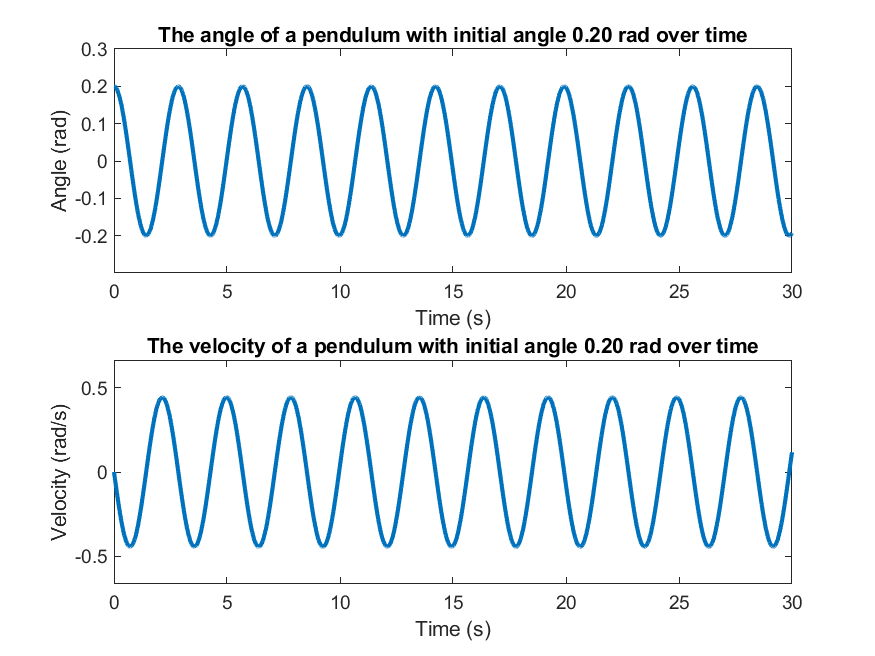
\includegraphics[width=14cm]{./output/assignment1/0.20_rad.png}
  \caption{Behavior of the pendulum with initial angle of 0.2 rad}
  \label{fig:figure1}
\end{figure}

\begin{figure}[H]
  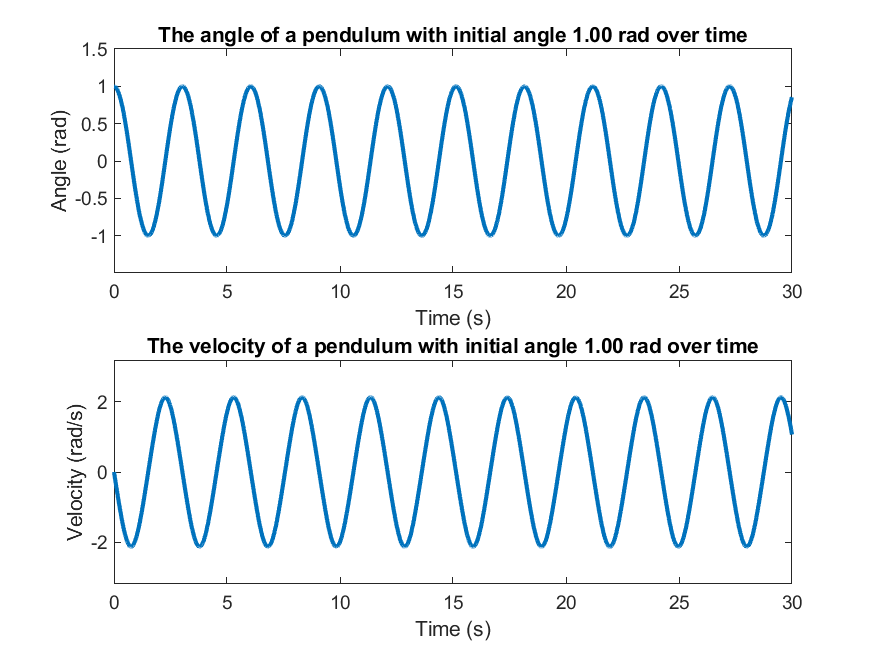
\includegraphics[width=14cm]{./output/assignment1/1.00_rad.png}
  \caption{Behavior of the pendulum with initial angle of 1 rad}
  \label{fig:figure2}
\end{figure}

\begin{figure}[H]
  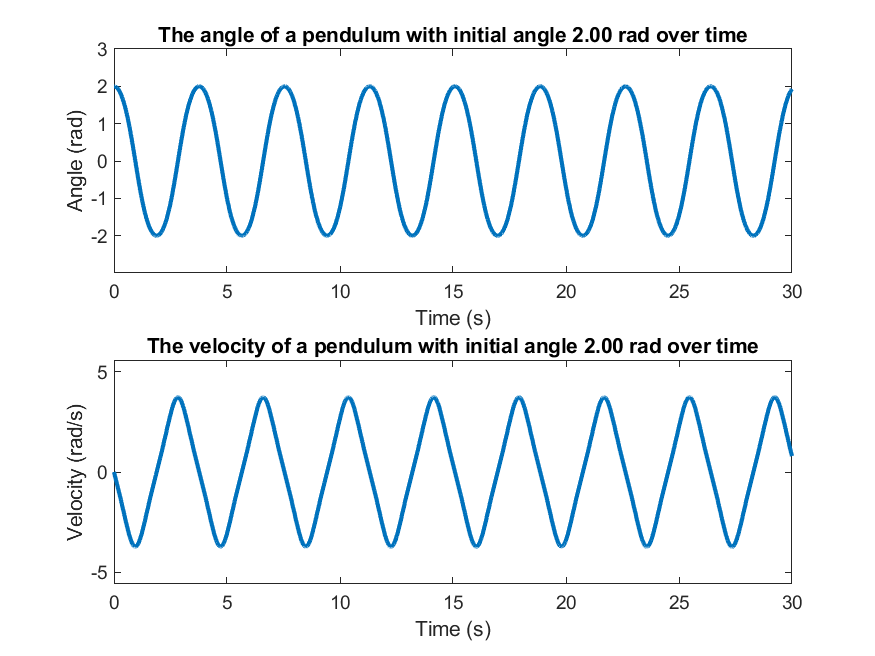
\includegraphics[width=14cm]{./output/assignment1/2.00_rad.png}
  \caption{Behavior of the pendulum with initial angle 2 rad}
  \label{fig:figure3}
\end{figure}

\begin{figure}[H]
  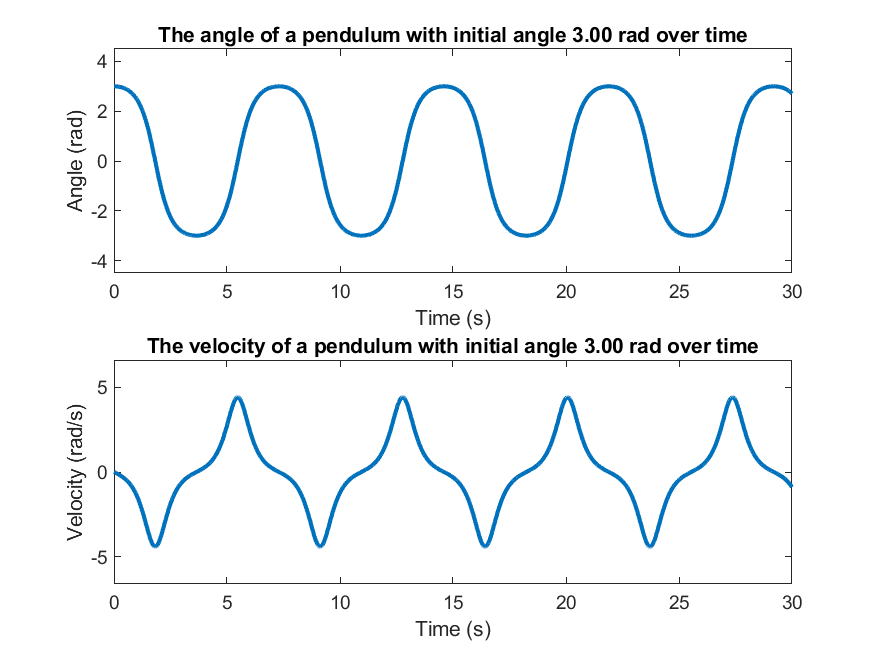
\includegraphics[width=14cm]{./output/assignment1/3.00_rad.png}
  \caption{Behavior of the pendulum with initial angle 3 rad}
  \label{fig:figure4}
\end{figure}

\begin{figure}[H]
  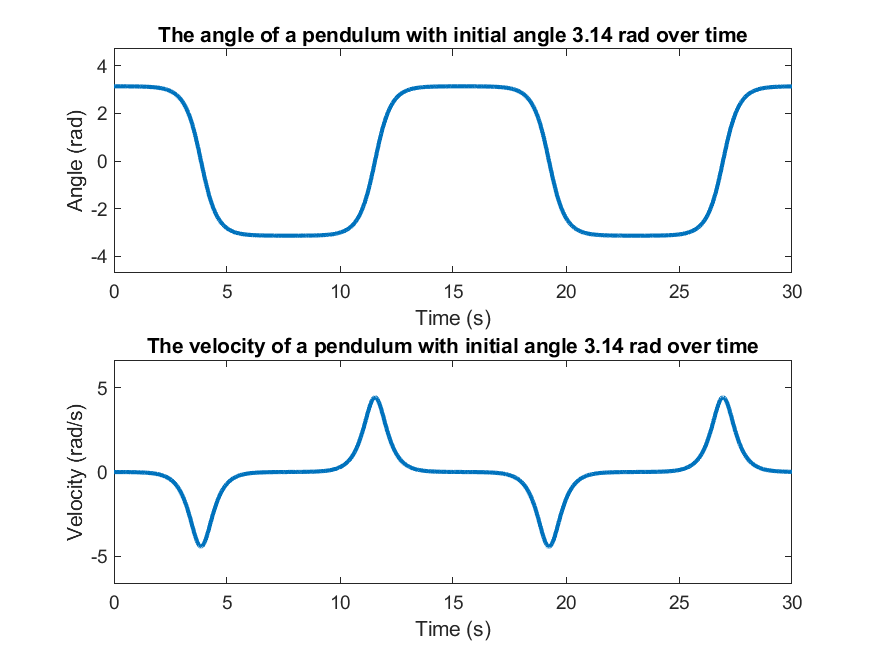
\includegraphics[width=14cm]{./output/assignment1/3.14_rad.png}
  \caption{Behavior of the pendulum with initial angle 3.14 rad}
  \label{fig:figure5}
\end{figure}

Using this data one can calculate the period of the pendulum under the given
initial angle $\theta_0$. The period describes how often a oscillation repeats itself.
Therefore it can be calculated by looking at how often the system reaches the same conditions.
As both the position and angle have the same period it is enough to look at one of them.
In the code this is done by getting all the times $t$ where the position of the pendulum
is at $\theta = 0 rad$. The provided "zerocrossing.m" method is used. To get the actual period
the time between these points is taken and averaged. They then have to be divided by 2 as the pendulum
is at point $\theta = 0$ twice in it's period (once with positive and once with negative velocity). These results
are then written into the \textit{comparison\_result} cell together with the analytical solution as well as the
the error between them. This result is later exported as a csv which can be seen here:

\csvautotabular{./output/assignment1/comparison_table.csv}

From the table it can be seen that the error between the two methods is very small at an angle of $\theta = 0 rad$

\section{Task 2}

This task uses the same building blocks as task one. The goal is now to precisely analyze the period of the
pendulum depending on the initial angle $\theta_0$ by producing a plot. The code to accomplish this looks like this:

\inputminted[linenos]{octave}{./matlab/assignment_2.m}

First the initial conditions have to be defined again. This time a lot more initial angles $\theta_0$ are
analyzed. To get the different angles the shorthand operator in line 1 is used to easily get values with
between $ 0.01 < \theta_0 < 0.9$ with $\Delta \theta_0 = 0.04 $ and $ 0.9 < \theta_0 < 0.999$ with $\Delta \theta_0 = 0.001 $ these represent the factors
of $\pi$ to be used. Those values are than each multiplied by $\pi$ using the standard matlab function 
\textit{arrayfun}\footnote{The function uses the function provided in the first argument on all the elements in the provided array (second parameter)
In the shown use case an inline method is again used for easy readability}\\
\\
Next the the result matrix \textit{periods} is initialized to store the produced periods in. The logic from
lines 9 to 33 follows the same pattern as explained in task 1. Instead of plotting each of the pendulums
behaviors instead the numerically found out period is put into the mentioned result matrix.\\
\\
This data is then plotted. The period compared ot the angles is plotted twice once as a continuous line and
once as dots, to show the sampling points (line 40). Additionally a plot at $\theta_0 = 0.01$ is added representing $T_0$\footnote{$\theta_0 = 0.01$ can be 
as the error is very small to the analytical solution we want to actually compare to} to compare the results with:

\begin{figure}[H]
  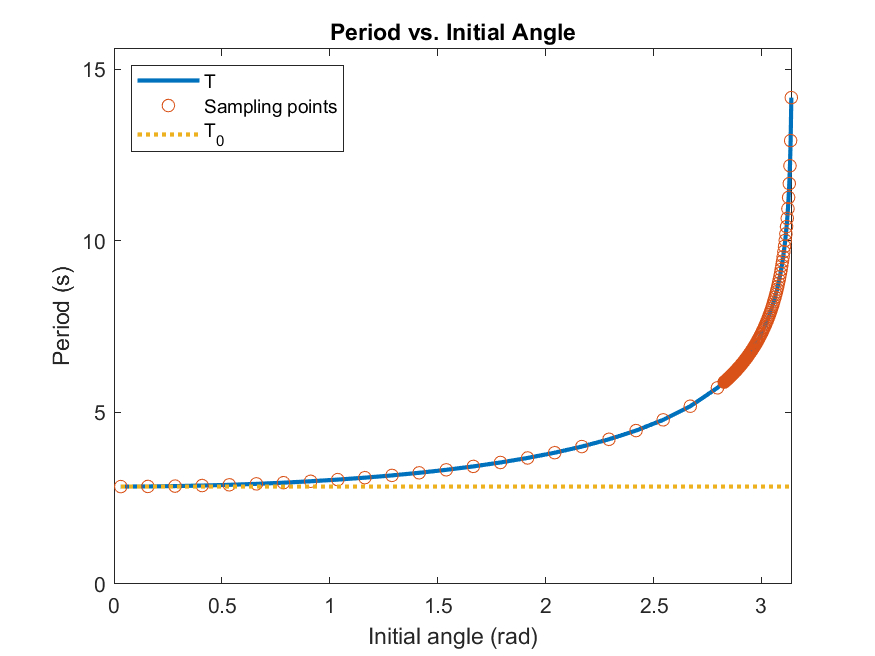
\includegraphics[width=14cm]{./output/assignment2.png}
  \caption{Period of the pendulum vs. initial angle}
  \label{fig:figure6}
\end{figure}

From the chart it can be seen that when the initial angle $\theta_0$ close to 0 the period $T$ assimptoaly approaches
the the theoretical solution $T_0$. On the other hand when $\theta_0$ approaches the period $T$ seems to rise exponentially
towards positive infinity. From initial appearance the the relationship seems to be exponential. This makes initutive sense if
thinking of the extreme case when $\theta_0 = \pi$. In this case the pendulum would stand exactly upright. Assuming there are
no external forces it would stay in that position as there is no component of the gravitational force acting lateral to the pendulum
and thus no acceleration would be applied to the pendulum. If the pendulum does not oscillate at all, the period is effectively infinite.
This is confirmed by the data in figure \ref{fig:figure6} as the period seems to approach infinity at $\theta_0 = \pi$

\section{Task 3}

Here the task is to implement a new custom differential equation to be solved by the same methods discussed in the two
previous tasks. The differential equation in question is about a heating situation of an indoor room. It is
described by the following equation:

\begin{equation}\label{eq_heating}
  \frac{d T_{in}(t)}{dt} = - \alpha(T_{in}(t) - T_{out}(t)) + c
\end{equation}

with $ T_{out} $ described by:

\begin{equation}\label{eq_tout}
  T_{out}(t) = T_{min} + \frac{T_{max} - T_{min}}{2}(1 + cos(2 \pi sin^2(\pi t/2)))
\end{equation}

The first thing to do was therefore to implement the given formulas as matlab methods. The implementation for
equation \ref{eq_tout} looks like this:

\inputminted[linenos]{octave}{./matlab/make_Tout.m}

As can be seen the method is again implemented in the factory pattern to avoid having to hand around globals.
The factory method gets as an input the two constants $T_{in}$ and $T_{out}$

The method itself is then quite straight forward as the equation is only a first order differential equation and
only one decimal number has to be returned opposed to a vector like in task 1. The full implementation of the 
equation can be done in one line and is essentially just a translation of the raw equation into matlab code (see line 14).\\
\\
The heating method is implemented in a similar way:

\inputminted[linenos]{octave}{./matlab/make_heating.m}

Again we provide the two constants $\alpha$ and $c$ in the factory method. Additionally an instance of the t\_out
method also needs to be provided as it is needed as part of the heating method. As equation \ref{eq_heating} is already
given in the form $\frac{dx}{dt}$ it already directly supplies the change within one time step, which is the value
needed for numerical integration. This again makes the implementation quite straight forward and it is only necessary
to translate the equation into matlab code directly.\\
\\
Finally the differential equation has to be solved numerically for different parameters and the result plotted:

\inputminted[linenos]{octave}{./matlab/assignment_3.m}

First all the constants $T_{min}$, $T_{max}$ and $T_{in 0}$ (Initial value of $T_{in}$). Then the differential
equations are defined. First the $T_{out}$ method is defined of which only one is needed as both $T_{min}$, ${T_{max}}$
are the same for all experiments. In contrast two hea ting methods need to be defined as the equation has to be solved
once for the heating being on and once for the heating being off: $c = 0 $ and $c = 25.5$\footnote{The value of $25.5$ was
estimated by adjusting and observing at what point the oscillations land around 21 $C^{\circ}$}. After obtaining\\
the methods both equations can be solved. 
\\
To obtain the $T_{out}$ values the \textit{arrayfun} is used again to call the method
for each of the timestamps. The last thing left is to plot the results which yields the following plot:

\begin{figure}[H]
  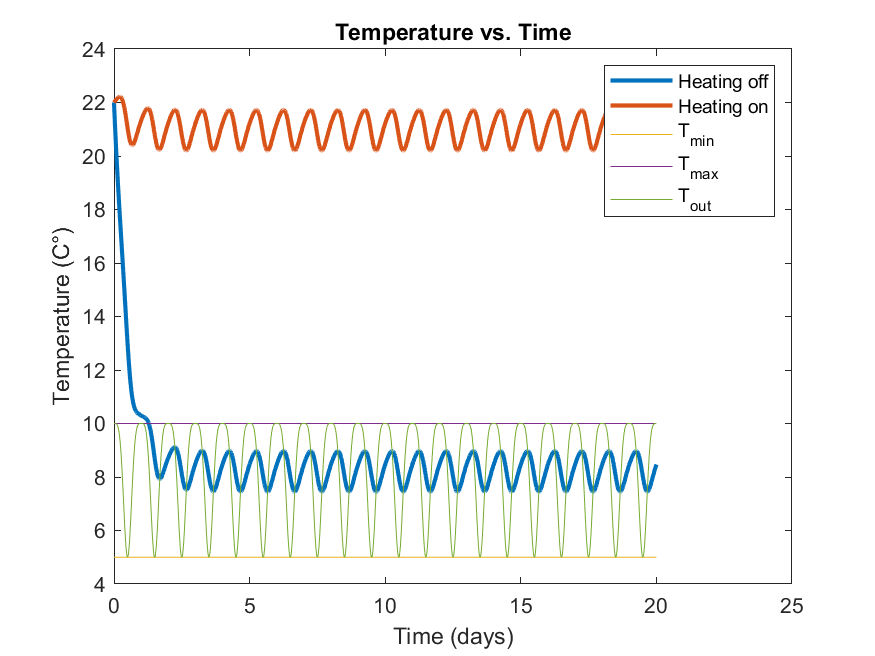
\includegraphics[width=14cm]{./output/assignment3.png}
  \caption{The temperature of the room over time}
  \label{fig:figure7}
\end{figure}

\printbibliography

\end{document}
